\documentclass[11pt,a4paper]{article}
\usepackage[OT4]{polski}
\usepackage[utf8]{inputenc}
\usepackage[inner=2.5cm,outer=2.5cm, tmargin=2.5cm,bmargin=2.5cm]{geometry}
\usepackage{amsmath}
\usepackage{relsize,amsfonts}
\usepackage{enumitem}
\usepackage{graphicx}

\newcommand\bigexists{%
  \mathop{\lower0.75ex\hbox{\ensuremath{%
    \mathlarger{\mathlarger{\mathlarger{\mathlarger{\exists}}}}}}}%
  \limits}
  
\newcommand\bigforall{%
  \mathop{\lower0.75ex\hbox{\ensuremath{%
    \mathlarger{\mathlarger{\mathlarger{\mathlarger{\forall}}}}}}}%
  \limits}
  
\title{Wspomaganie Decyzji w Warunkach Ryzyka\\\large \medskip Projekt: WDWR 25406\\}
\author{Krzysztof Rudnicki 307585}
\date{\today}

\begin{document}

\maketitle

\section*{Treść zadania}
\addcontentsline{toc}{section}{Treść zadania}
Rozważmy następujące zagadnienie planowania produkcji:

\begin{itemize}
  \item Przedsiębiorstwo wytwarza 4 produkty P1,...,P4 na następujących maszynach: 4 szlifierkach, 2 wiertarkach pionowych, 3 wiertarkach poziomych, 1 frezarce i 1 tokarce. Wymagane czasy produkcji 1 sztuki produktu (w godzinach) w danym procesie obróbki zostały przedstawione w poniższej tabeli:\\
  \begin{center}
  \begin{tabular}{l*{4}{c}}
  	\hline
              			& P1 & P2 & P3 & P4 \\
	\hline
	Szlifowanie 		& 0,4 & 0,6 & - & - \\
	Wiercenie pionowe   & 0,2 & 0,1 & - & 0,6 \\
	Wiercenie poziome 	& 0,1 & - & 0,7 & -  \\
	Frezowanie  	 	& 0,06 & 0,04 & - & 0,05 \\
	Toczenie	     	& - & 0,05 & 0,02 & - \\
	\hline
	\end{tabular}
	\end{center}

  \item Dochody ze sprzedaży produktów (w zł/sztukę) określają składowe wektora $\mathbf{R} = (R_{1},...,R_{4})^{T}$. Wektor $\mathbf{R}$ opisuje 4-wymiarowy rozkład \textit{t}-Studenta z 4 stopniami swobody, którego wartości składowych zostały zawężone do przedziału $[5;12]$. Wektor wartości oczekiwanych $\mu$ oraz macierz kowariancji $\Sigma$ niezawężonego rozkładu \textit{t}-Studenta są następujące:
  \begin{displaymath}
\mathbf{\mu} = 
 \begin{pmatrix}
  9 \\ 8 \\ 7 \\ 6 \\  
 \end{pmatrix},
 \mathbf{\Sigma} = 
 \begin{pmatrix}
  16 & -2 & -1 & -3 \\
  -2 & 9 & -4 & -1 \\ 
  -1 & -4 & 4 & 1 \\
  -3 & -1 & 1 & 1 \\  
 \end{pmatrix}
  \end{displaymath}
  
  \item Istnieją ograniczenia rynkowe na liczbę sprzedawanych produktów w danym miesiącu:
  \begin{center}
  \begin{tabular}{l*{4}{c}}
  	\hline
              			& P1 & P2 & P3 & P4 \\
	\hline
	Styczeń 			& 200 & 0 & 100 & 200 \\
	Luty   				& 300 & 100 & 200 & 200 \\
	Marzec 				& 0 & 300 & 100 & 200  \\
	\hline
	\end{tabular}
	\end{center}
	
	\item Jeżeli sprzedaż danego produktu przekracza 80 procent ilości jaką może wchłonąć rynek, jego dochód spada o 20 procent.
	
	\item Istnieje możliwość składowania do 200 sztuk każdego produktu w danym czasie w cenie 1 zł/sztukę za miesiąc. W chwili obecnej (grudzień) w magazynach znajduje się 0 sztuk każdego produkt. Istnieje wymaganie, aby tyle pozostało również pod koniec marca.
	
	\item Przedsiębiorstwo pracuje 6 dni w tygodniu w systemie dwóch zmian. Każda zmiana trwa 8 godzin. Można założyć, że każdy miesiąc składa się z 24 dni roboczych.
\end{itemize}

\section*{Polecenia}
\addcontentsline{toc}{section}{Polecenia}
\begin{enumerate}
  \item Zaproponować jednokryterialny model wyboru w warunkach ryzyka z wartością oczekiwaną jako miarą zysku. Wyznaczyć rozwiązanie optymalne.
  \item Jako rozszerzenie powyższego zaproponować dwukryterialny model zysku i ryzyka ze średnią jako miarą zysku i średnią różnicą Giniego jako miarą ryzyka. Dla decyzji $\mathbf{x}\in Q$ średnia różnica Giniego jest definiowana jako $\Gamma(\mathbf{x})=\frac{1}{2}\sum_{t'=1}^{T}\sum_{t"=1}^{T}\lvert r_{t'}(\mathbf{x})-r_{t"}(\mathbf{x})\rvert p_{t'}p_{t"}$, gdzie $r_{t'}(\mathbf{x})$ oznacza realizację dla scenariusza t, $p_{t}$ prawdopodobieństwo scenariusza t.
  \begin{enumerate}
    \item Wyznaczyć obraz zbioru rozwiązań efektywnych w przestrzeni zysk-ryzyko.
    \item Wskazać rozwiązania efektywne minimalnego ryzyka i maksymalnego zysku. Jakie odpowiadają im wartości w przestrzeni ryzyko-zysk?
    \item Wybrać trzy dowolne rozwiązania efektywne. Sprawdzić, czy zachodzi pomiędzy nimi relacja dominacji stochastycznej pierwszego rzędu. Wyniki skomentować, odnieść do ogólnego przypadku.
  \end{enumerate}
\end{enumerate}

\section{Jednokryterialny model wyboru}
Jednokryterialny model wyboru w warunkach ryzyka ma umożliwić wybór rozwiązania optymalnego ze względu na maksymalizację wartości oczekiwanej zysku. Wartość oczekiwana ma być określana na podstawie scenariuszy wygenerowanych z rozkładu \textit{t}-Studenta o parametrach podanych w treści zadania. Przyjęto, że wszystkie scenariusze mają takie same prawdopodobieństwo.
\subsection{Parametry modelu}
W tabeli \ref{tab:param} zestawiono wszystkie przyjęte parametry modelu razem z opisami. Takie samo nazwy przyjęto podczas implementacji modelu. W przypadku wektorów oraz macierzy parametrów w nawiasach kwadratowych podano ich rozmiar odwołując się do parametrów liczbowych.
\begin{table}[ht!]
\caption{Tabela zawierająca parametry modelu jednokryterialnego}
\label{tab:param}
\begin{tabular}{lp{9cm}}
	\hline
	Nazwa parametru      & Opis \\
	\hline
	nMachType & Ilość typów maszyn (procesów) dostępnych w fabryce \\
nMonth & Ilość miesięcy uwzględnionych w symulacji  \\
nProdType & Ilość typów produktów \\
nScenarios & Ilość scenariuszy wygenerowanych do symulacji \\
machines[nMachType] & Wektor typów maszyn (procesów)\\
months[nMonth] & Wektor miesięcy symulacji\\
products[nProdType] & Wektor typów produktów\\
machineCount[nMachType] & Wektor ilości maszyn danego typu\\
prodTime[nMachType][nProdType] & macierz czasów produkcji danego produktu na danej maszynie \\
maxInMonth[nMonth][nProdType] & macierz maksymalnej ilości produktów, jakie można sprzedać w danym miesiącu\\
nHours & Ilość godzin pracy fabryki w miesiącu\\
mu[nProdType] & Wektor wartości oczekiwanych rozkładu t-Studenta do generacji scenariuszy\\
sigma [nProdType][nProdType] & Macierz kowariancji dla rozkłady t-Studenta\\ 
sellProfit[nScenarios][nProdType] & Macierz wygenerowanych sceniariuszy dochodów ze sprzedaży produktów\\
storageCost & Koszt trzymania jednej sztuki produktu w magazynie przez miesiąc \\
storageMax[nProdType] & Wektor maksymalnej pojemności magazynu dla każdego typu produktu \\
storageStart[nProdType] & Wektor ilości początkowej produktów w magazynie \\
	\hline
\end{tabular}
\end{table}

\subsection{Zmienne decyzyjne}
Zmienne decyzyjne są kontrolowanymi przez decydenta, kluczowymi dla problemu wartościami. Celem systemu jest dobranie przez solver takich wartości tych zmiennych, które pozwolą na osiągnięcie najlepszego rozwiązania zadania. W tabeli \ref{tab:var} przedstawiono zmienne decyzyjne wykorzystane w modelu wraz z opisami. Zastosowano konwencję nazw identyczną, jak w przypadku parametrów modelu.

\begin{table}[ht!]
\caption{Tabela zawierająca zmienne decyzyjne modelu}
\label{tab:var}
\begin{tabular}{lp{7.5cm}}
	\hline
	Nazwa zmiennej      & Opis \\
	\hline
	produce[nMonth][nProdType] & Macierz zawierające ilości wytwarzanych sztuk danego typu produktu w danym miesiącu \\
	sell[nMonth][nProdType] & Macierz zawierająca ilości sprzedawanych sztuk danego typu produktu w danym miesiącu \\
	stock[nMonth][nProdType] & Macierz zawierająca ilości sztuk danego typu produktu znajdujących się w magazynie w danym miesiącu \\
	workTime[nMonth][nMachType][nProdType] & Macierz zawierająca czas pracy każdej maszyny dla każdego typu produktu w kazdym miesiącu \\
	if80prec[nMonth][nProdType] & Macierz zmiennych binarnych (1 jeśli sprzedaż danego produktu w danym miesiącu przekroczyła 80\% wartości maksymalnej, 0 - w przeciwnym wypadku)\\
	lowerProfit[nScenarios][nMonth][nProdType] & Macierz przechowująca kwoty, jaką należy odjąć od zysków z poszczególnych typów produktów w poszczególnych miesiącach, ze względu na przekroczenie 80\% pojemności rynku. Zmienna niezbędna do wyeliminowania obecności zmiennej binarnej w funkcji oceny\\
	\hline
\end{tabular}
\end{table}

\subsection{Ograniczenia}
Z punktu widzenia projektowania modelu, najważniejsze jest prawidłowe dobranie przedstawionych założeniach ograniczeń. Zidentyfikowano następujące ograniczenia modelu:
\begin{itemize}
\item Ograniczenie dolne wartości zmiennych decyzyjnych – wartości nie mogą być mniejsze od zera:
	\begin{equation}
	\bigforall_{\substack{
			m \in months \\ 
			p \in products \\
			mc \in machines}} workTime[m][mc][p] >=0
	\end{equation}
	\begin{equation}
	\bigforall_{\substack{
			m \in months \\ 
			p \in products}} produce[m][p] >=0
	\end{equation}
	\begin{equation}
	\bigforall_{\substack{
			m \in months \\ 
			p \in products}} sell[m][p] >=0
	\end{equation}
	\begin{equation}
	\bigforall_{\substack{
			m \in months \\ 
			p \in products}} stock[m][p] >=0
	\end{equation}
	\begin{equation}
	\bigforall_{\substack{
			i \in scenarios \\
			m \in months \\ 
			p \in products}} lowerProfit[i][m][p] >=0
	\end{equation}

\item Ograniczenie ilości jednocześnie pracujących maszyn - Ze względu na to, że każda pojedyncza maszyna może pracować w ciągu miesiąca \textit{nHours} godzin, to dla każdego typu maszyny, czas ich pracy nie może przekroczyć wartości iloczynu ilości maszyn danego typu oraz czasu \textit{nHours}.
	\begin{equation}
		\bigforall_{\substack{
			m \in months\\ 
			mc \in machines}}  \sum_{p \in products}
		(workTime[m][mc][p] <= machineCount[mc]*nHours)
	\end{equation}
	\item Ograniczenie definiujące czas pracy maszyn - czas pracy danego typu maszyny to iloczyn ilości wyprodukowanych sztuk danego produktu i czasu trwania danego procesu technologicznego dla jednej sztuki:
	\begin{equation}
		\bigforall_{\substack{
			m \in months\\ 
			mc \in machines\\
			p \in products}} workTime[m][mc][p] == produce[m][p]*prodTime[mc][p]
	\end{equation}
	\item Ograniczenie rynkowe maksymalnej sprzedaży w danym miesiącu:
	\begin{equation}
		\bigforall_{\substack{
			m \in months\\ 
			p \in products}} sell[m][p] == maxInMonth[m][p]
	\end{equation}
	
	\item Ograniczenia ustawiające zmienną binarną po przekroczeniu 80 procent pojemności rynku:
	\begin{equation}
		\bigforall_{\substack{
			m \in months\\ 
			p \in products}}  sell[m][p] <= 0.8*maxInMonth[m][p] + 1000000 * if80prec[m][p]
	\end{equation}
	\begin{equation}
		\bigforall_{\substack{
			m \in months\\ 
			p \in products}} sell[m][p] >= 0.8*maxInMonth[m][p] * if80prec[m][p]
	\end{equation}
	
	\item Ograniczenia linearyzujące wpływ zmiennej binarnej na funkcje celu:
	\begin{equation}
		\bigforall_{\substack{
			i \in scenarios\\			
			m \in months\\ 
			p \in products}} lowerProfit[i][m][p] <= 1000000 * if80prec[m][p]
	\end{equation}
	\begin{equation}
		\bigforall_{\substack{
			i \in scenarios\\			
			m \in months\\ 
			p \in products}} lowerProfit[i][m][p] <= 0.2 * sell[m][p]*sellProfit[i][p]
	\end{equation}
	\begin{multline}
		\bigforall_{\substack{
			i \in scenarios\\			
			m \in months\\ 
			p \in products}} 0.2 * sell[m][p]*sellProfit[i][p] - lowerProfit[i][m][p] +\\ 1000000 * if80prec[m][p] <= 1000000;
	\end{multline}
	
	\item Ograniczenie sprzedaż do ilości sztuk wyprodukowanych oraz znajdujących się w magazynie. Dla pierwszego miesiąca ma ono postać:
	\begin{equation}
		\bigforall_{\substack{
			m \in months\\ 
			p \in products}} sell[m][p] <= produce[m][p]+storageStart[p]
	\end{equation}
	Dla każdego następnego miesiąca:
	\begin{equation}
		\bigforall_{\substack{
			m \in months\\ 
			p \in products}} sell[m][p] <= produce[m][p] + stock[m-1][p]
	\end{equation}
	
	\item Ograniczenie definiujące ilość produktów pozostających w magazynach na następny miesiąc, jako sumę sztuk wyprodukowanych i będących w magazynie na początku tego miesiąca pomniejszoną o ilość sprzedaną w tym miesiącu. Dla pierwszego miesiąca:
	\begin{equation}
		\bigforall_{\substack{
			m \in months\\ 
			p \in products}} stock[m][p]==(produce[m][p] + storageStart[p])-sell[m][p]
	\end{equation}
	Dla każdego następnego miesiąca:
	\begin{equation}
		\bigforall_{\substack{
			m \in months\\ 
			p \in products}} stock[m][p]==(produce[m][p] + stock[m-1][p])-sell[m][p]
	\end{equation}

\end{itemize}
\subsection{Funkcja celu}
Funkcja celu dla modelu jednokryterialnego to maksymalizacja wartości oczekiwanej zysku dla wszystkich scenariuszy. Dla każdego scenariusza została przyjęta funkcja zysku w postaci
\begin{multline}
\bigforall_{\substack{
			i<nScernarios\\ 
			i \in N}}  
	profit[i] =\sum_{m \in months} \sum_{p \in products}
		(sell[m][p]\cdot sellProfit[i][p] \\ -lowerProfit[i][m][p]-stock[m][p]*storageCost)
\end{multline}
 


\subsection{Implementacja modelu}
\subsubsection{Generacja scenariusz dochodów ze sprzedaży}
Dochody ze sprzedaży poszczególnych produktów są określone wektorem losowym określonym w treści zadania. Do wygenerowania wektorów opisujących konkretne scenariusze sprzedaży wykorzystano pakiet MASS dla języka R. Skrypt drukujący wektory do pliku został napisany w środowisku R Studio IDE. Załącznik 1 to wspomniany skrypt - \textit{t-student.R}. Do potrzeby symulacji wygenerowano 1000 scenariuszy.

\subsubsection{Model}
Rozwiązanie zadania zaimplementowano w całości przy pomocy programu IBM ILOG CPLEX Optimization Studio przy wykorzystaniu solvera CPLEX. Nazwy parametrów oraz zmiennych decyzyjnych pokrywają się z nazwami opisanymi w tabelach \ref{tab:param} i \ref{tab:var}. Załącznik 2 to plik \textit{wdwr17421-1.dat}, który definiuje parametry modelu. Załącznik 3 to plik \textit{wdwr17421-1.mod}, który wczytuje parametry modelu, definiuje zmienne decyzyjne, funkcję oceny oraz ograniczenia modelu. Dla przyśpieszenia implementacji modelu przyjęto, że kolejne miesiące, produkty oraz procesy technologiczne będą opisane liczbami naturalnymi.  Miesiące ponumerowane są w kolejności występowania, produkty według indeksu przy literze P w nazwie, a procesy technologiczne w następujące kolejności:
\begin{enumerate}
\item Szlifowanie,
\item Wiercenie pionowe,
\item Wiercenie poziome,
\item Frezowanie,
\item Toczenie.
\end{enumerate}

\subsection{Rozwiązanie}
Optymalne rozwiązanie maksymalizacji wartości oczekiwanej zysku zostało obliczone przez solver CPLEX. Optymalny zysk wyniósł około 26023,63 zł. Wynik taki jest osiągany dla następujących wartości zmiennych decyzyjnych:
\begin{displaymath}
\mathbf{sell} = 
 \begin{pmatrix}
  320 & 0 & 160 & 240 \\
  700 & 320 & 500 & 0 \\ 
  0 & 800 & 600 & 320 \\  
 \end{pmatrix},
 \mathbf{if80prec} = 
 \begin{pmatrix}
  0 & 1 & 0 & 0 \\
  1 & 0 & 1 & 1 \\ 
  1 & 1 & 1 & 0 \\  
 \end{pmatrix},
\end{displaymath}
\begin{displaymath}
\mathbf{stock} = 
 \begin{pmatrix}
  0 & 50 & 0 & 0 \\
  0 & 0 & 0 & 0 \\ 
  50 & 50 & 50 & 50 \\  
 \end{pmatrix},
 \mathbf{produce} = 
 \begin{pmatrix}
  270 & 0 & 110 & 190 \\
  700 & 270 & 500 & 0 \\ 
  50 & 850 & 650 & 370 \\  
 \end{pmatrix} 
\end{displaymath}

Macierze z czasami pracy maszyn dla poszczególnych typów produktów zostały przedstawione oddzielnie dla każdego miesiąca:
\begin{displaymath}
 \mathbf{workTime[1]} =
 \begin{pmatrix}
  108 & 0 & 0 & 0 \\
  54 & 0 & 0 & 114 \\ 
  27 & 0 & 77 & 0 \\
  16.2 & 0 & 0 & 9.5 \\
  0 & 0 & 2.2 & 0 \\  
 \end{pmatrix},
 \mathbf{workTime[2]} =
 \begin{pmatrix}
  280 & 162 & 0 & 0 \\
  140 & 27 & 0 & 0 \\ 
  70 & 0 & 350 & 0 \\
  42 & 10.8 & 0 & 0 \\ 
  0 & 13.5 & 10 & 0 \\
 \end{pmatrix},
\end{displaymath}
\begin{displaymath}
 \mathbf{workTime[3]} =
 \begin{pmatrix}
  20 & 510 & 0 & 0 \\
  10 & 85 & 0 & 222 \\ 
  5 & 0 & 455 & 0 \\
  3 & 34 & 0 & 18.5 \\ 
  0 & 42.5 & 13 & 0 \\
 \end{pmatrix}
\end{displaymath}

Macierzy lowerProfit nie przedstawiono w raporcie ze względu na jej wielkość. Pełne wyniki działania solvera dołączono do raportu jako załącznik 4.
\subsection{Wnioski}
Z przeprowadzonej sytuacji wynika, że możliwości produkcyjne fabryki przekraczają pojemność rynku. W celu maksymalizacji w niektórych miesiącach opłaca się sprzedawać poszczególne produkty, nawet po przekroczeniu 80\% pojemności rynku. Nie ma potrzeby magazynowania produktów, poza wymaganym minimum.

\section{Model dwukryterialny zysku i ryzyka}
\subsection{Model zadania}
Model przedsiębiorstwa pozostał w całości taki, jak w pierwszej części zadania. Miarą zysku jest wartość oczekiwana, czyli w przypadku równie prawdopodobnych scenariuszy - średnia. Miarą ryzyka w danym zadaniu jest średnia różnica Giniego wyrażająca się wzorem:
\begin{equation}
\Gamma(\mathbf{x})=\frac{1}{2}\sum_{t'=1}^{T}\sum_{t"=1}^{T}\lvert r_{t'}(\mathbf{x})-r_{t"}(\mathbf{x})\rvert p_{t'}p_{t"}, 
\end{equation}
gdzie $r_{t'}(\mathbf{x})$ oznacza realizację dla scenariusza t, a $p_{t}$ - prawdopodobieństwo scenariusza t.

Zgodnie z przyjętymi w projekcie oznaczeniami wyrażenie określające miarę ryzyka będzie wyglądało następująco:
\begin{equation}
giniRisk = \frac{1}{2}\cdot\sum_{t1 \in scenarios}\sum_{t2 \in scenarios} \lvert profit[t1]-profit[t2] \rvert \cdot \frac{1}{nScenarios} \cdot \frac{1}{nScenarios} 
\end{equation}

\subsection{Model preferencji}
Model preferencji został zbudowany na podstawie wymaganego poziomu średniej przy minimalizacji ryzyka.
\begin{equation}
avgProfit<minAvgProfit
\end{equation}
\begin{equation}
minimize giniRisk
\end{equation}
minAvgProfit jest dodatkowym parametrem modelu. Załączniki 5 i 6 to pliki z paramtrami i modelem zadania dwukryterialnego wyboru - pliki źródłowe dla solvera CPLEX. 

\subsection{Zbiór rozwiązań efektywnych w przestrzeni ryzyko-zysk}
Rysunek \ref{fig:profit-risk} przedstawia rozwiązania efektywne modelu w przestrzeni ryzyko-zysk. Niebieskie trójkąty przedstawiają rozwiązanie efektywne dla różnych wartości wymaganego poziomu zysku. Ze względu na możliwości obliczeniowe komputera rozwiązania 52 równo odległe rozwiązania, każe biorące pod uwagę 30 scenariuszy. Wprowadzono ograniczenie czasu solvera poświęconego jednemu rozwiązania do 5 min. Obliczenia zajęły ponad 3 godziny. Załączniki 7 i 8 to pliki parametrów oraz modelu wraz ze skryptem dla solvera CPLEX, służące do uzyskania rozwiązań. Kolorem żółtym oznaczono rozwiązanie maksymalnego zysku oraz minimalnego ryzyka. Odpowiadające im wartości zawarte są w tabeli \ref{tab:min-max}. 
\begin{figure}[ht!]
\centering
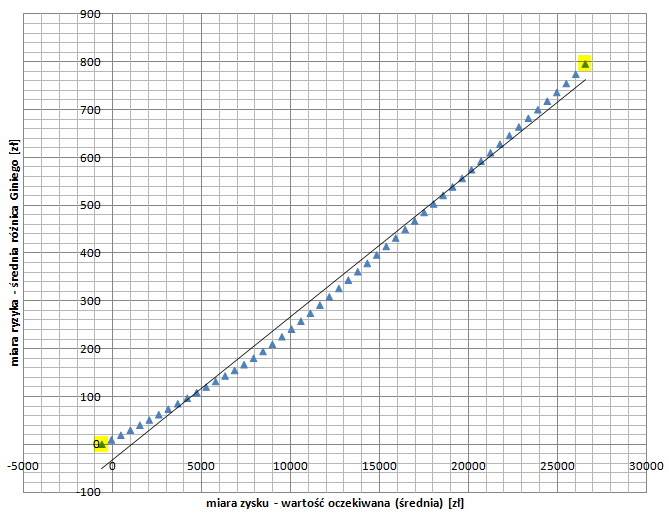
\includegraphics[width=0.8\textwidth]{graphics/results-minAvgProfit-marker}
\caption{Obraz zbioru rozwiązań efektywnych w przestrzeni ryzyko-zysk}
\label{fig:profit-risk}
\end{figure}

\subsection{Rozwiązania efektywne minimalnego ryzyka i maksymalnego zysku}

Na wykresie \ref{fig:profit-risk} kolorem żółtym oznaczono rozwiązania maksymalnego zysku oraz minimalnego ryzyka. Odpowiadające im wartości w przestrzeni ryzyko zysk zawarte są w tabeli \ref{tab:min-max}.

\begin{table}[ht!]
\label{tab:min-max}
  \caption{Rozwiązania maksymalnego zysku i minimalnego ryzyka}
  \centering
  \begin{tabular}{l*{4}{c}}
  
  	\hline
              			& Miara zysku & Miara ryzyka \\
	\hline
	Maksymalizacja zysku	& 26553.9 zł & 796.113 zł \\
	Minimalizacja ryzyka   	& -600.00 zł & 0.0 zł \\ 
	\hline
	
	\end{tabular}
	\end{table}
	
Rozwiązanie zadania jednokryterialnego maksymalizacji zysku wiąże się maksymalizacją ryzyka, natomiast zadanie minimalizacji ryzyka, bez ograniczeń na miarę zysku powoduje stratę (zysk ujemny) spowodowaną brakiem sprzedaży oraz kosztami utrzymania minimalnego stanu magazynu.

\subsection{Sprawdzenie dominacji stochastycznej wybranych rozwiązań efektywnych}

W celu sprawdzenia dominacji stochastycznej pierwszego rzędu (FSD) wybrano 3 rozwiązania efektywne modelu. Zostały oznaczone literami A, B, C. Wartości średniego zysku oraz miary ryzyka odpowiadające tym rozwiązaniom zostały przedstawione w tabeli \ref{tab:abc}. Wybrano rozwiązanie, które były do siebie najbardziej zbliżone pod względem średniej zysku. Jej wartość różniła się o około 500 zł. Załączniki 9 i 10 to pliki parametrów oraz modelu wraz ze skryptem dla solvera CPLEX, służące do wygenerowania informacji o zysku i ryzyku dla poszczególnych scenariuszy.

\begin{table}[ht!]
  \label{tab:abc}
  \caption{Rozwiązania wybrane do analizy dominacji FSD}
  \centering
  \begin{tabular}{lccc}
  	\hline
              			& A & B & C \\
	\hline
	Ograniczenie minimalnego zysku	& 25488.1 zł & 26020.5 zł & 26552.9 zł\\
	Średni zysk   	& 25488.3 zł & 26020.6 zł & 26553.9 zł\\
	Miara ryzyka   	& 755.133 zł & 774.872 zł & 796.113 zł\\ 
	\hline
	\end{tabular}
\end{table}


Aby sprawdzić dominację wzajemną dominację rozwiązań w sensie FSD narysowano odwrotne dystrybuanty dla obydwu kryteriów. Rysunek \ref{fig:FSD-profit} przedstawia wykres odwrotnej dystrybuanty rozkładu średniego zysku pomiędzy scenariuszami dla 3 wybranych rozwiązań efektywnych. Z wykresu można odczytać, że rozwiązanie C dominuje rozwiązania A i B w sensie FSD, tzn. że dla każdego scenariusza miara zysku w przypadku decyzji C jest większa niż w przypadku decyzji A i B. Rozwiązanie B dominuje w sensie FSD rozwiązanie A.

\begin{figure}[ht!]
\centering
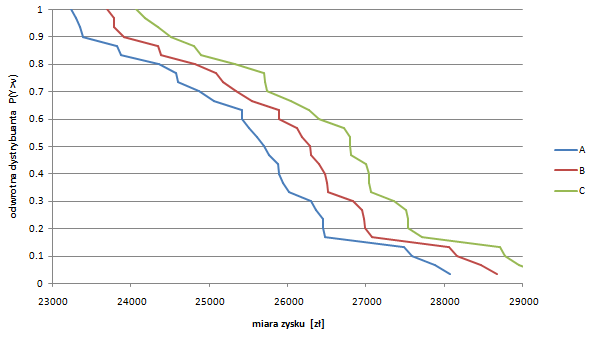
\includegraphics[width=\textwidth]{graphics/results-FSD-profit}
\caption{Odwrotna dystrybuanta rozkładu średniego zysku między scenariuszami}
\label{fig:FSD-profit}
\end{figure}

Rysunek \ref{fig:FSD-risk} to wykres odwrotnej dystrybuanty rozkładu średniego różnicy Giniego jako miary ryzyka pomiędzy scenariuszami dla tych samych 3 rozwiązań efektywnych. Ze względu na miarę ryzyka rozwiązanie A dominuje rozwiązania B, C, natomiast rozwiązanie B nie dominuje "ściśle" rozwiązania C. Powodem jest przecinanie się dystrybuant w miejscu oznaczonym na żółto na wykresie na rysunku \ref{fig:FSD-profit}.

\begin{figure}[ht!]
\centering
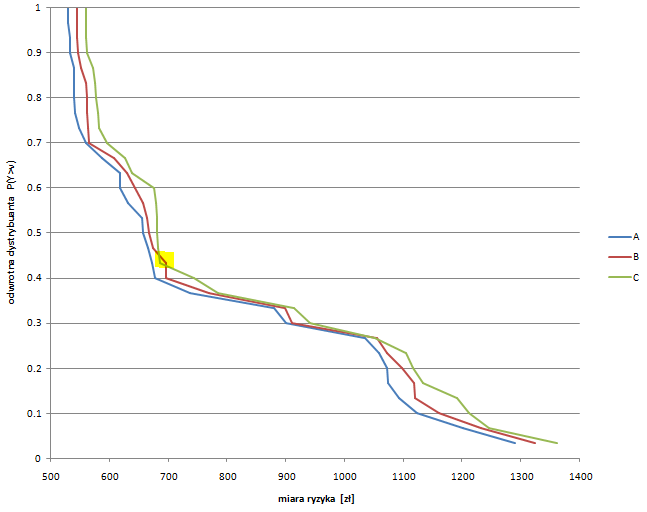
\includegraphics[width=0.95\textwidth]{graphics/results-FSD-risk}
\caption{Odwrotna dystrybuanta rozkładu średniej różnicy Giniego między scenariuszami}
\label{fig:FSD-risk}
\end{figure}


\clearpage
%%% SPIS TABEL %%%
% \phantomsection
\addcontentsline{toc}{chapter}{\listtablename}
\listoftables

%%% SPIS ZAŁĄCZNIKÓW %%%
\addcontentsline{toc}{section}{Spis załączników} 
\section*{Spis załączników}
\begin{enumerate}
\item t-Student.R - skrypt generujący wektory opisujące dochód ze sprzedaży produktów w poszczególnych scenariuszy,
\item wdwr17421-1.dat - plik definiujący parametry modelu jednokryterialnego,
\item wdwr17421-1.mod - plik implementujący model jednokryterialny,
\item wdwr17421-1.log - pełne wyniki działania solvera dla modelu jednokryterialnego,
\item wdwr17421-2.dat - plik definiujący parametry modelu dwukryterialnego,
\item wdwr17421-2.mod - plik implementujący model dwukryterialny,
\item wdwr17421-3.dat - plik definiujący parametry modelu dwukryterialnego,
\item wdwr17421-3.mod - plik implementujący model oraz skrypt do uzyskania obrazu rozwiązań w przestrzeni ryzyko-zysk,
\item wdwr17421-4.dat - plik definiujący parametry modelu,
\item wdwr17421-4.mod - plik implementujący model oraz skrypt do uzyskania danych do analizy dominacji FSD.
\end{enumerate}



\end{document}